\documentclass[11pt]{article}

\usepackage[a4paper,margin=1in]{geometry}
\usepackage[T1]{fontenc}
\usepackage{lmodern}
\usepackage{microtype}
\usepackage{amsmath,amssymb}
\usepackage{graphicx}
\usepackage{booktabs}
\usepackage{tabularx}
\usepackage{array}
\usepackage{float}
\usepackage{subcaption}
\usepackage{enumitem}
\usepackage{xcolor}
\usepackage{hyperref}

\hypersetup{
  colorlinks=true,
  linkcolor=blue!50!black,
  urlcolor=blue!60!black,
  citecolor=blue!50!black
}

\setlength{\parindent}{0pt}
\setlength{\parskip}{0.55em}
\renewcommand{\arraystretch}{1.15}

\newcommand{\repoinfo}{\href{https://github.com/arfinzz/CLAP-Special-Topic-DBMS}{\texttt{https://github.com/arfinzz/CLAP-Special-Topic-DBMS}}}
\newcommand{\dataset}[1]{\texttt{#1}}

\title{\textbf{Reproducing and Extending CLAP for Zero-Shot Audio Classification}\\
\large Project Report}

\author{
Shuvam Chakraborty (2024MCS2004)\\
Arfin Khan (2024MCS2001)\\
Bhuvnesh Kumar (2023MCS2011)
}

\date{April 22, 2026}

\begin{document}
\maketitle

\begin{center}
\small COL868 Special Topics in DBMS\\
\vspace{0.75em}

\fcolorbox{black}{blue!5}{%
\parbox{0.92\linewidth}{%
\centering
\normalsize \textbf{Code Repository:} \repoinfo
}%
}
\end{center}

\begin{abstract}
This project studies \emph{zero-shot audio classification} using CLAP
(Contrastive Language-Audio Pretraining). The main task is to classify an input
audio clip without task-specific supervised training by comparing its audio
embedding against text embeddings generated from class prompts. Our work is not
just a benchmark rerun: it is a reproduction-plus-extension study with a fully
verified evaluation pipeline. We rebuilt the benchmark workflow, stabilized the
environment in WSL2, ran the complete benchmark suite over
\dataset{ESC-50}, \dataset{UrbanSound8K}, \dataset{GTZAN}, and
\dataset{FSDD}, and produced reproducibility artifacts including dataset
verification, checkpoint manifests, run manifests, and acceptance checks. The
final run uses the official LAION CLAP implementation together with the stronger
\dataset{630k-audioset-best.pt} checkpoint, so the most accurate description of
the project is an \emph{improved-checkpoint reproduction with extensions}. The
main empirical findings are that CLAP transfers very well to environmental
sound recognition, remains reasonably strong on urban sound and music genre
classification, fails clearly on spoken-digit recognition, and does not obtain
reliable gains from prompt ensembling.
\end{abstract}

\section{Introduction and Motivation}

The original CLAP idea is compelling because it extends the CLIP-style
contrastive paradigm from image-text learning to audio-text learning. Instead
of training a dedicated classifier for each downstream dataset, CLAP learns a
shared embedding space in which audio clips and natural-language descriptions
can be compared directly. This creates the possibility of \emph{zero-shot
transfer}: predicting classes by prompt matching rather than supervised
retraining.

Our project was designed as a reproduction-plus-extension study rather than a
single-number rerun. We wanted to answer the following questions:

\begin{itemize}[leftmargin=1.25em]
  \item How well does CLAP transfer across environmental sound, urban sound,
  music genre, and speech-like tasks?
  \item Can the published benchmark-style setup be rebuilt in a verifiable
  environment?
  \item How sensitive are zero-shot results to prompt wording?
  \item Does prompt ensembling, inspired by CLIP-style prompt ensembling in
  vision, improve robustness?
  \item What happens when CLAP is tested on a narrow speech classification task
  rather than only sound and music tasks?
\end{itemize}

The project therefore had two main goals:
\begin{itemize}[leftmargin=1.25em]
  \item reproduce the paper-style zero-shot benchmark on
  \dataset{ESC-50}, \dataset{UrbanSound8K}, and \dataset{GTZAN};
  \item extend the study with a new dataset, richer metrics, prompt
  sensitivity analysis, prompt ensembling, and reproducibility tooling.
\end{itemize}

The final verified run uses the stronger
\dataset{630k-audioset-best.pt} checkpoint rather than the exact original
checkpoint configuration associated with the paper comparison. Because of that,
the work should be described honestly as:

\begin{itemize}[leftmargin=1.25em]
  \item a \textbf{full benchmark reproduction with an improved checkpoint};
  \item plus \textbf{extension experiments and analysis}.
\end{itemize}

\section{Background and Task Formulation}

\subsection{Main Task}

The central task in this project is \textbf{zero-shot audio classification}.
Given an audio clip and a set of class labels, the model must predict the
correct class \emph{without} task-specific supervised training on that dataset.

Instead of learning a dataset-specific classifier head, we convert class labels
into natural-language prompts and compare the audio embedding against text
embeddings. Conceptually, this means that prediction is reduced to a retrieval
problem in a shared embedding space.

\subsection{Paper Idea and CLAP Intuition}

CLAP learns two encoders jointly:
\begin{itemize}[leftmargin=1.25em]
  \item an audio encoder $f_a(x)$;
  \item a text encoder $f_t(y)$,
\end{itemize}
where $x$ is an audio clip and $y$ is a text description.

During contrastive training, matched audio-text pairs are brought closer in the
embedding space while mismatched pairs are pushed apart. After pretraining,
downstream classification becomes possible by expressing each class as text and
retrieving the class whose text embedding is most similar to the audio
embedding.

If $z_a = f_a(x)$ and $z_t = f_t(y)$, then the similarity score used in the
zero-shot stage is cosine similarity:

\begin{equation}
s(x, y) = \cos(z_a, z_t) = \frac{z_a \cdot z_t}{\lVert z_a \rVert \lVert z_t \rVert}.
\end{equation}

For a class set $C = \{c_1, \dots, c_K\}$, we build prompts
$p(c_1), \dots, p(c_K)$ and predict:

\begin{equation}
\hat{y} = \arg\max_k \; s\bigl(x, p(c_k)\bigr).
\end{equation}

\subsection{Prompting and Prompt Ensembling}

Prompt phrasing matters. A class such as \dataset{dog barking} can be written
as:
\begin{itemize}[leftmargin=1.25em]
  \item ``this is a sound of dog barking'',
  \item ``the audio contains dog barking'',
  \item ``a recording of dog barking'',
\end{itemize}
and each phrasing yields a slightly different text embedding.

This project therefore studies not only single-prompt inference but also prompt
ensembling. Let $T=\{t_1,\dots,t_M\}$ be the prompt family and let
$p_{k,m}=t_m(c_k)$ be the $m$-th prompt template for class $c_k$. Then:

\begin{equation}
z_i = f_a(x_i), \qquad q_{k,m} = f_t(p_{k,m}).
\end{equation}

For a single prompt template, the class score is:

\begin{equation}
s_k^{(m)} = \cos(z_i, q_{k,m}).
\end{equation}

Uniform prompt ensembling averages prompt embeddings:

\begin{equation}
q_k^{\text{ens}} = \frac{1}{M} \sum_m q_{k,m}.
\end{equation}

Weighted prompt ensembling uses:

\begin{equation}
q_k^{\text{ens}} = \sum_m w_m q_{k,m}, \qquad \sum_m w_m = 1.
\end{equation}

The final prediction is then:

\begin{equation}
\hat{y}_i = \arg\max_k \cos\bigl(z_i, q_k^{\text{ens}}\bigr).
\end{equation}

We implemented both uniform and entropy-weighted ensembling. One of the most
important negative findings of the project is that this strategy does not
produce reliable gains.

\section{Method}

\subsection{System Overview}

The project uses two repositories together:
\begin{itemize}[leftmargin=1.25em]
  \item \dataset{clap-official}:
  the official LAION CLAP implementation, which provides the actual
  \dataset{laion\_clap} model code;
  \item \dataset{clap-reimpl}:
  our experiment layer, which provides dataset loading, prompt generation,
  metric computation, run wrappers, figures, manifests, and the final report.
\end{itemize}

The evaluation pipeline follows the same high-level procedure across datasets:
\begin{enumerate}[leftmargin=1.4em]
  \item prepare audio paths, labels, and metadata for the dataset;
  \item generate text prompts from a prompt family suited to the domain;
  \item compute CLAP audio embeddings and CLAP text embeddings;
  \item compute similarity scores and obtain ranked predictions;
  \item aggregate results into metrics, figures, JSON reports, and summary
  tables.
\end{enumerate}

The design intentionally separates:
\begin{itemize}[leftmargin=1.25em]
  \item model implementation,
  \item dataset preparation,
  \item benchmark logic,
  \item reporting and figures,
  \item reproducibility logging.
\end{itemize}

This separation mattered practically because it allowed us to stabilize the
environment, change checkpoints, and add new datasets without rewriting the
core model code.

\subsection{Dataset Abstractions and Prompt Families}

The main benchmark runner is
\dataset{scripts/analysis/run\_zeroshot\_metrics.py}. Its design centers on a
\dataset{DatasetBundle} abstraction containing:
\begin{itemize}[leftmargin=1.25em]
  \item dataset key,
  \item display name,
  \item root directory,
  \item prompt family,
  \item class names,
  \item audio files,
  \item numeric labels,
  \item dataset-specific metadata.
\end{itemize}

Supported datasets are:
\begin{itemize}[leftmargin=1.25em]
  \item \dataset{esc50},
  \item \dataset{urbansound8k},
  \item \dataset{gtzan},
  \item \dataset{fsdd}.
\end{itemize}

Three prompt families are used:
\begin{itemize}[leftmargin=1.25em]
  \item \dataset{sound},
  \item \dataset{music},
  \item \dataset{speech}.
\end{itemize}

Datasets are assigned families as follows:
\begin{itemize}[leftmargin=1.25em]
  \item \dataset{ESC-50} and \dataset{UrbanSound8K}: \dataset{sound};
  \item \dataset{GTZAN}: \dataset{music};
  \item \dataset{FSDD}: \dataset{speech}.
\end{itemize}

This matters because prompt phrasing produces visibly different results on some
datasets, especially \dataset{GTZAN} and \dataset{FSDD}.

\subsection{Caching and Generated Outputs}

Audio and text embeddings are cached under
\dataset{outputs/embeddings/<dataset>/}. The cache contains:
\begin{itemize}[leftmargin=1.25em]
  \item \dataset{audio\_embeddings.npy},
  \item \dataset{labels.npy},
  \item \dataset{audio\_files.json},
  \item prompt-specific text embedding arrays,
  \item ensemble embeddings.
\end{itemize}

Caching made repeated evaluation practical and significantly reduced rerun time
during debugging and extension experiments.

For each dataset, the pipeline generates:
\begin{itemize}[leftmargin=1.25em]
  \item metrics JSON,
  \item confusion matrix,
  \item reliability diagram,
  \item per-class accuracy plot,
  \item prompt sensitivity plot,
  \item ensemble comparison plot.
\end{itemize}

At the global level, it also generates:
\begin{itemize}[leftmargin=1.25em]
  \item summary CSV tables,
  \item summary plots,
  \item run manifests,
  \item acceptance reports.
\end{itemize}

\subsection{Environment and Engineering Notes}

The final verified run used:
\begin{itemize}[leftmargin=1.25em]
  \item WSL2 with Ubuntu 22.04,
  \item Python 3.10,
  \item \dataset{torch 2.4.1+cu121},
  \item \dataset{numpy 1.26.4},
  \item \dataset{transformers 4.30.0},
  \item checkpoint \dataset{630k-audioset-best.pt}.
\end{itemize}

One implementation detail mattered for stability: a small NumPy compatibility
shim was added so that the official CLAP data path worked correctly in the
final environment. This should be treated as part of the method rather than as
an irrelevant implementation accident.

\subsection{Datasets and Evaluation Scope}

\begin{table}[H]
\centering
\small
\resizebox{\textwidth}{!}{%
\begin{tabular}{lccccl}
\toprule
Dataset & Samples & Classes & Domain & Track & Default Prompt Family \\
\midrule
\dataset{ESC-50} & 2000 & 50 & Environmental sound & Baseline + Extension & sound \\
\dataset{UrbanSound8K} & 8732 & 10 & Urban sound & Baseline + Extension & sound \\
\dataset{GTZAN} & 999 & 10 & Music genre & Baseline + Extension & music \\
\dataset{FSDD} & 3000 & 10 & Spoken digits & Extension only & speech \\
\bottomrule
\end{tabular}%
}
\caption{Datasets used in the final verified study.}
\end{table}

Two experiment tracks were run:

\begin{itemize}[leftmargin=1.25em]
  \item \textbf{Baseline track:}
  \dataset{ESC-50}, \dataset{UrbanSound8K}, and \dataset{GTZAN};
  \item \textbf{Extension track:}
  \dataset{ESC-50}, \dataset{UrbanSound8K}, \dataset{GTZAN}, and
  \dataset{FSDD}.
\end{itemize}

The baseline track reproduces the original benchmark-style dataset suite in the
verified setup. The extension track evaluates the improved checkpoint, richer
metrics, prompt sensitivity, and prompt ensembling.

\subsection{Reproducibility and Dataset Preparation}

The final artifact set includes:
\begin{itemize}[leftmargin=1.25em]
  \item dataset verification,
  \item checkpoint manifest generation,
  \item baseline and extension manifests,
  \item GTZAN preparation manifest,
  \item final acceptance check.
\end{itemize}

One special preparation step was required for \dataset{GTZAN}. The raw archive
was converted from \dataset{.au} to \dataset{.wav}, then normalized to the
expected benchmark form by removing the known problematic sample
\dataset{jazz.00054.wav}. The final acceptance report passed with
\dataset{all\_ok = true}.

\section{Evaluation Setup and Metrics}

\subsection{Metrics}

This project extends the original reporting style by adding several metrics
beyond top-1 accuracy.

\subsubsection*{Top-1 Accuracy}

\begin{equation}
\text{Accuracy} = \frac{1}{N} \sum_i \mathbf{1}[\hat{y}_i = y_i].
\end{equation}

\subsubsection*{Macro-F1}

For each class $k$, let precision be $P_k$ and recall be $R_k$:

\begin{equation}
F1_k = \frac{2 P_k R_k}{P_k + R_k},
\qquad
\text{Macro-F1} = \frac{1}{K} \sum_k F1_k.
\end{equation}

Macro-F1 treats all classes equally and is useful when performance is uneven
across classes.

\subsubsection*{Balanced Accuracy}

\begin{equation}
\text{Balanced Accuracy} = \frac{1}{K} \sum_k \text{Recall}_k.
\end{equation}

\subsubsection*{Top-5 Accuracy}

\begin{equation}
\text{Top-5} = \frac{1}{N} \sum_i \mathbf{1}[y_i \in \text{top-5 ranked classes for sample } i].
\end{equation}

\subsubsection*{Mean Reciprocal Rank (MRR)}

If $\text{rank}_i$ is the rank of the correct class for sample $i$, then:

\begin{equation}
\text{MRR} = \frac{1}{N} \sum_i \frac{1}{\text{rank}_i}.
\end{equation}

\subsubsection*{Expected Calibration Error (ECE)}

\begin{equation}
\text{ECE} = \sum_b \frac{|B_b|}{N} \left| \text{acc}(B_b) - \text{conf}(B_b) \right|,
\end{equation}

where $B_b$ is the set of predictions in confidence bin $b$.

\subsubsection*{Prompt Sensitivity Score}

Prompt sensitivity captures the spread between best and worst prompt
performance:

\begin{equation}
\text{PSS} = \text{best prompt score} - \text{worst prompt score}.
\end{equation}

\subsection{What the Metric Suite Adds}

The richer metric set is important because it reveals behavior that plain
accuracy would hide:
\begin{itemize}[leftmargin=1.25em]
  \item \dataset{GTZAN} has moderate top-1 accuracy but very strong Top-5
  behavior, meaning the model often ranks the correct genre near the top.
  \item \dataset{FSDD} has poor top-1 accuracy but noticeably higher Top-5,
  suggesting weak partial awareness rather than complete collapse.
  \item \dataset{UrbanSound8K} behaves better under balanced accuracy than a
  single top-1 number might suggest.
\end{itemize}

\section{Results}

\subsection{Main Benchmark Results}

\begin{table}[H]
\centering
\small
\begin{tabular}{lcccccc}
\toprule
Dataset & Accuracy & Macro-F1 & Bal. Acc. & Top-5 & MRR & ECE \\
\midrule
\dataset{ESC-50} & 0.9150 & 0.9120 & 0.9150 & 0.9935 & 0.9499 & 0.8833 \\
\dataset{UrbanSound8K} & 0.7747 & 0.7786 & 0.7905 & 0.9612 & 0.8582 & 0.6382 \\
\dataset{GTZAN} & 0.6086 & 0.5878 & 0.6089 & 0.9570 & 0.7529 & 0.4857 \\
\dataset{FSDD} & 0.1053 & 0.0629 & 0.1053 & 0.5677 & 0.3133 & 0.0003 \\
\bottomrule
\end{tabular}
\caption{Final zero-shot performance on the four evaluated datasets.}
\end{table}

The results show a clear hierarchy of difficulty:
\begin{itemize}[leftmargin=1.25em]
  \item \dataset{ESC-50} is the strongest result and confirms that CLAP
  transfers well to environmental sound events.
  \item \dataset{UrbanSound8K} remains strong, though prompt wording affects it
  more noticeably.
  \item \dataset{GTZAN} is moderate rather than dominant, with confusion among
  semantically close genres.
  \item \dataset{FSDD} is the clearest failure case and shows that general
  audio-language pretraining is not sufficient for fine-grained spoken-digit
  recognition in zero-shot mode.
\end{itemize}

\begin{figure}[H]
\centering
\begin{subfigure}[t]{0.48\textwidth}
  \centering
  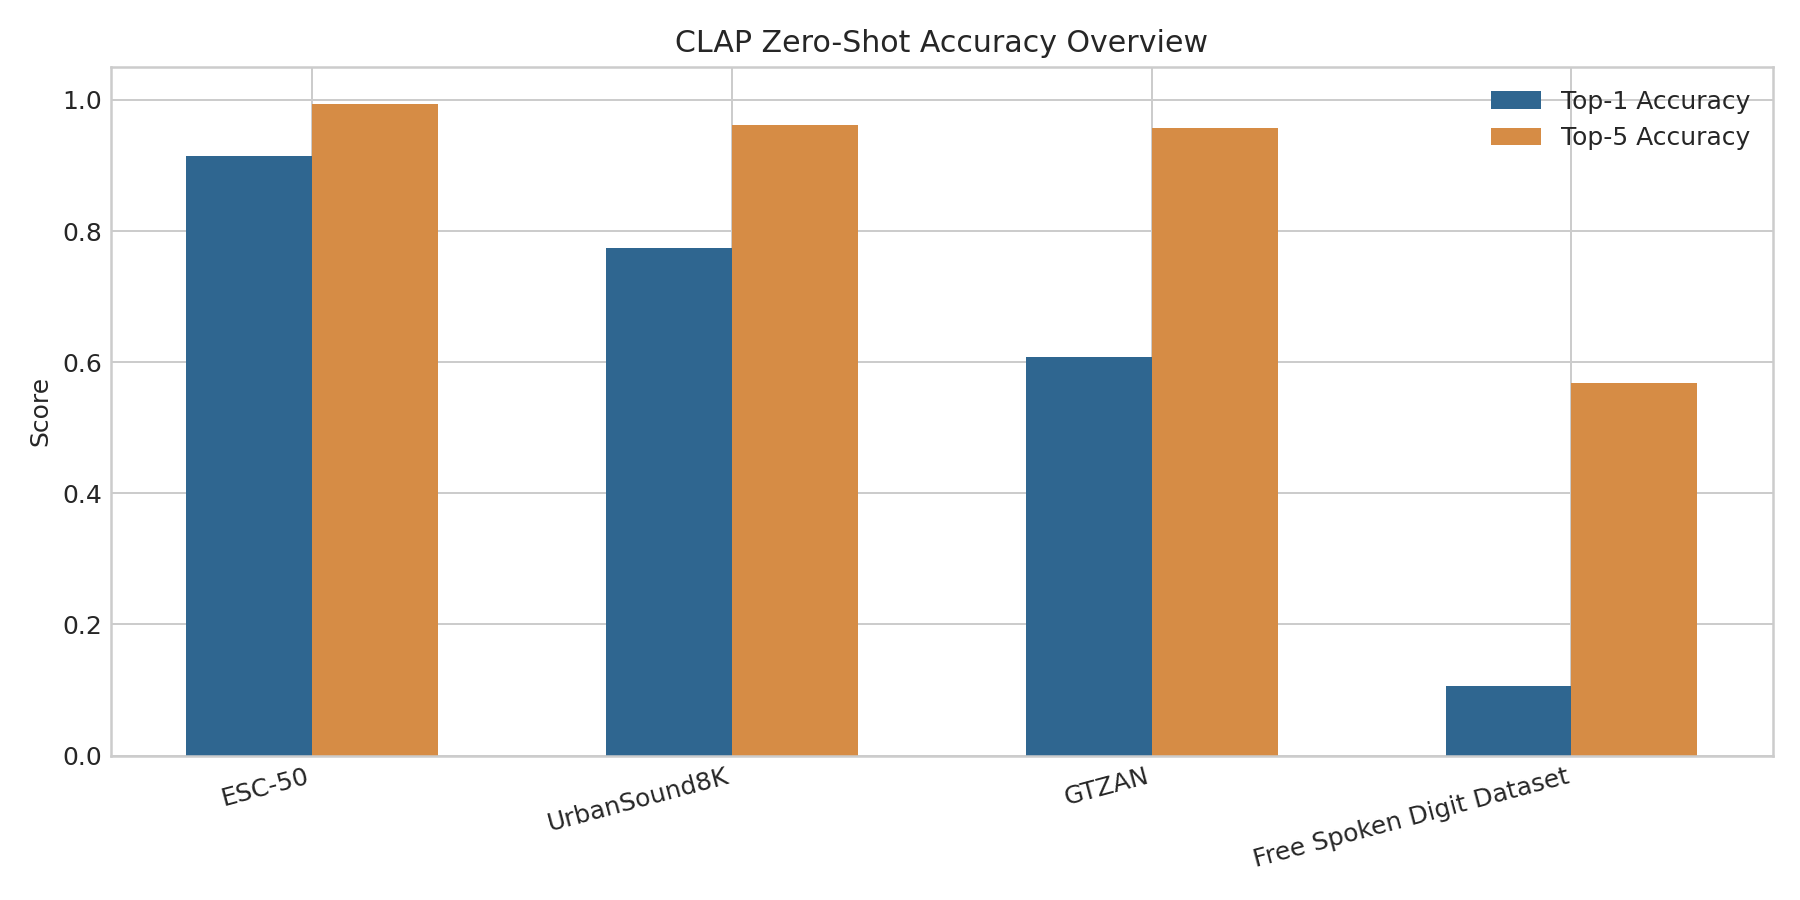
\includegraphics[width=\linewidth]{assets/summary/accuracy_overview.png}
  \caption{Accuracy overview across datasets.}
\end{subfigure}
\hfill
\begin{subfigure}[t]{0.48\textwidth}
  \centering
  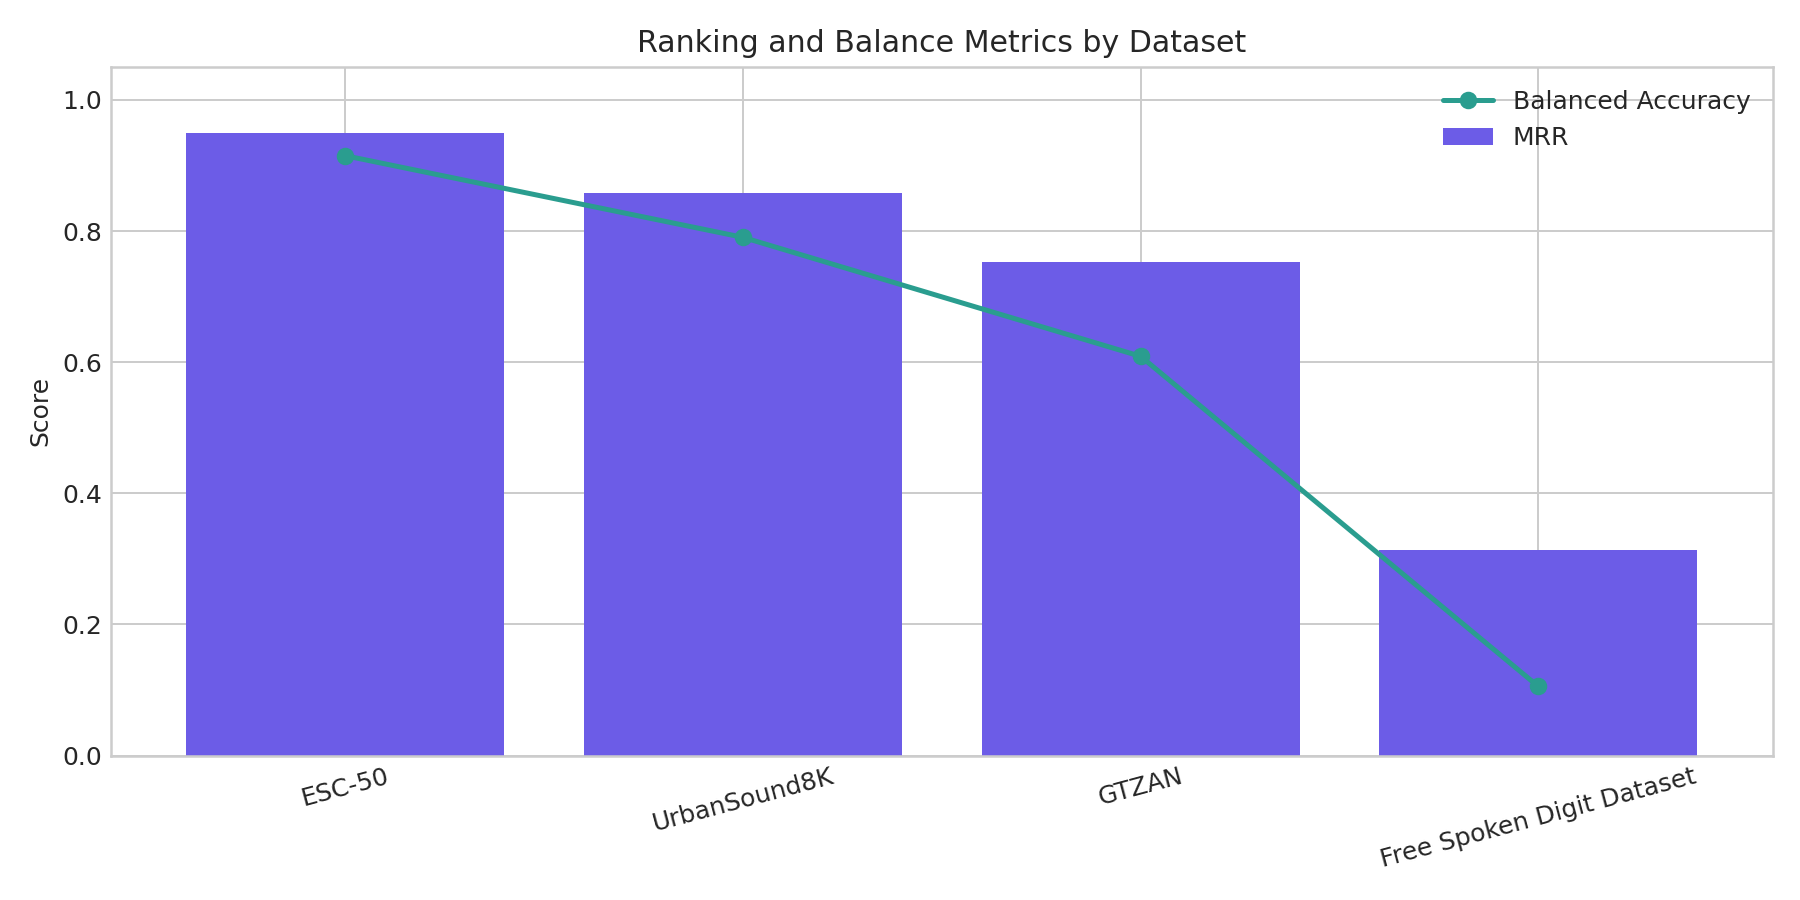
\includegraphics[width=\linewidth]{assets/summary/ranking_balance_overview.png}
  \caption{Ranking and balance behavior.}
\end{subfigure}
\caption{Summary plots generated from the final evaluation pipeline.}
\end{figure}

\subsection{Improvements Beyond the Original Benchmark}

This project includes three main improvements beyond a plain rerun:
\begin{enumerate}[leftmargin=1.4em]
  \item addition of \dataset{FSDD};
  \item addition of richer metrics;
  \item addition of prompt ensembling analysis.
\end{enumerate}

\subsubsection*{Improvement 1: FSDD}

\dataset{FSDD} was added as a speech-focused diagnostic dataset. Its purpose is
to test whether a general audio-language representation transfers to a
fine-grained speech classification task.

Result:
\begin{itemize}[leftmargin=1.25em]
  \item top-1 accuracy: \dataset{0.1053}
\end{itemize}

Interpretation:
\begin{itemize}[leftmargin=1.25em]
  \item performance is close to random for a 10-class task;
  \item this is strong evidence that CLAP is weak on zero-shot spoken-digit
  recognition.
\end{itemize}

\subsubsection*{Improvement 2: Richer Metrics}

The richer evaluation makes several important things visible that plain
accuracy would hide:
\begin{itemize}[leftmargin=1.25em]
  \item \dataset{GTZAN} is much stronger as a ranking model than as a hard
  classifier.
  \item \dataset{UrbanSound8K} has better balanced-accuracy behavior than its
  single accuracy number suggests.
  \item \dataset{FSDD} has weak top-1 transfer but nontrivial ranking
  structure.
\end{itemize}

\subsubsection*{Improvement 3: Prompt Ensembling}

Prompt ensembling was inspired by CLIP-style prompt ensembling in image-text
models. We implemented:
\begin{itemize}[leftmargin=1.25em]
  \item uniform averaging;
  \item entropy-weighted averaging.
\end{itemize}

\begin{table}[H]
\centering
\small
\begin{tabular}{lcccc}
\toprule
Dataset & Worst Prompt & Best Prompt & Uniform Ensemble & $\Delta$ vs Best \\
\midrule
\dataset{ESC-50} & 0.9150 & 0.9265 & 0.9270 & +0.0005 \\
\dataset{UrbanSound8K} & 0.7747 & 0.8106 & 0.7989 & -0.0117 \\
\dataset{GTZAN} & 0.5966 & 0.6647 & 0.6537 & -0.0110 \\
\dataset{FSDD} & 0.0740 & 0.1057 & 0.0757 & -0.0300 \\
\bottomrule
\end{tabular}
\caption{Prompt ensembling results.}
\end{table}

\begin{figure}[H]
\centering
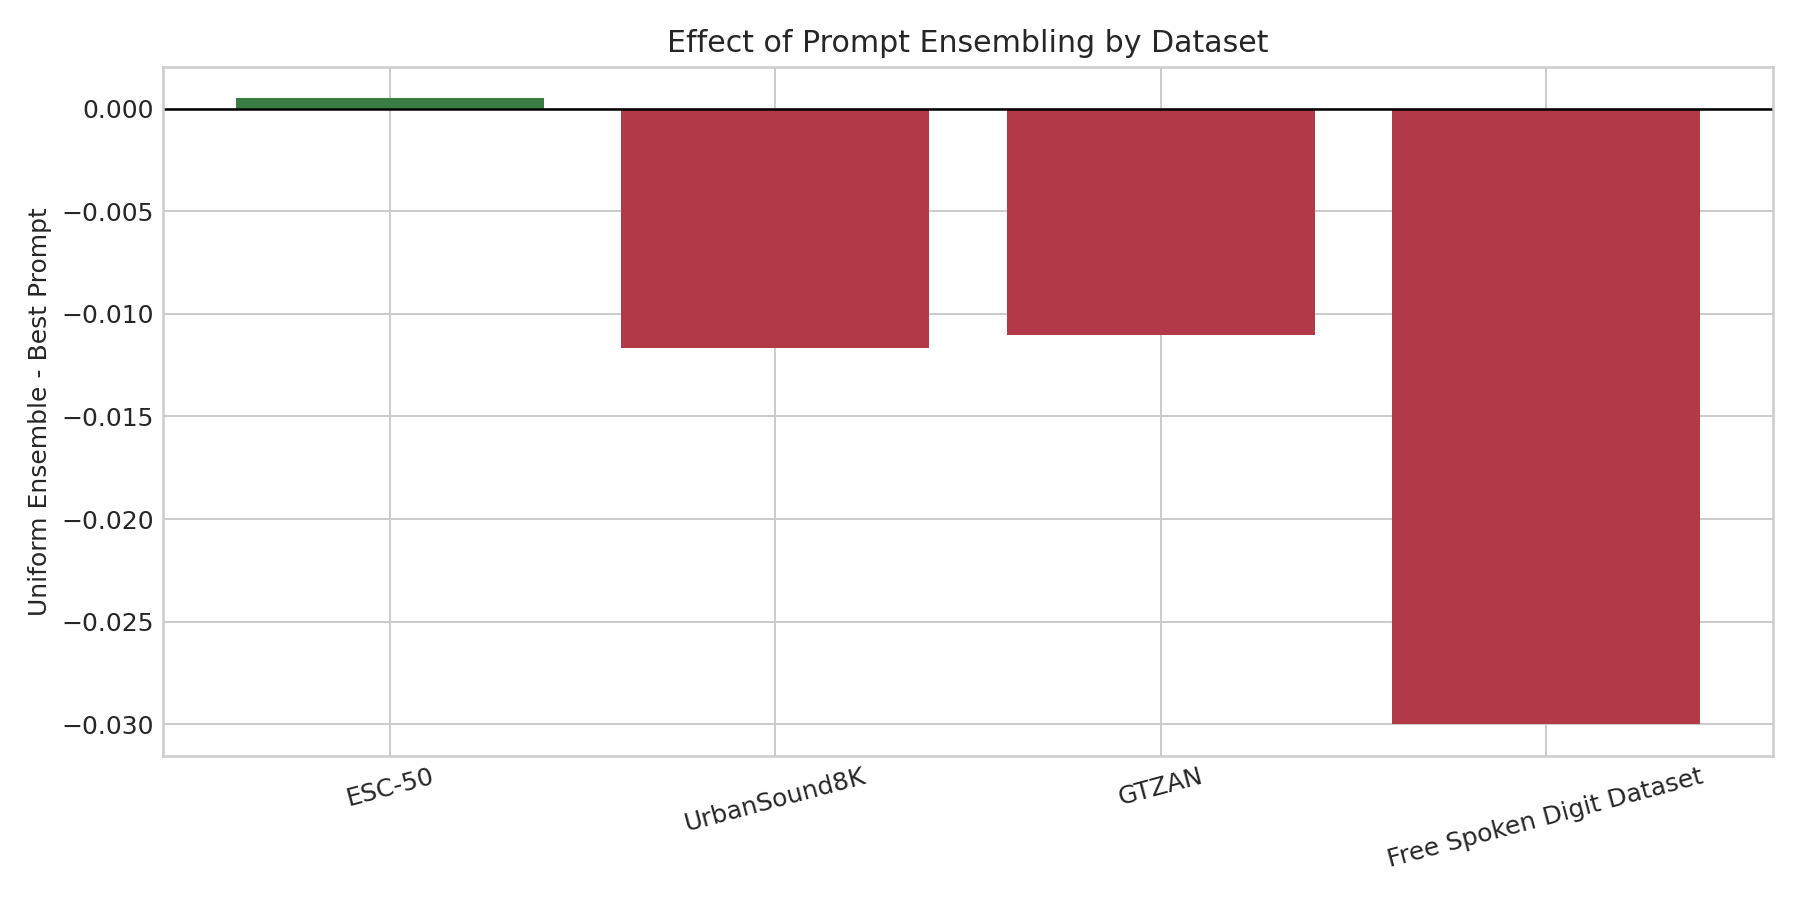
\includegraphics[width=0.72\textwidth]{assets/summary/ensemble_delta.png}
\caption{Effect of prompt ensembling relative to the best single prompt.}
\end{figure}

Prompt ensembling is the strongest negative result in the project. It gives
only a tiny gain on \dataset{ESC-50} and reduces performance on
\dataset{UrbanSound8K}, \dataset{GTZAN}, and \dataset{FSDD}. The
entropy-weighted ensemble did not improve over the uniform ensemble in the
final runs because the weights effectively collapsed to near-uniform values.
In practice, CLAP did not separate the prompt variants strongly enough for the
weighting strategy to matter.

\subsection{Visual Diagnostics}

\subsubsection*{Ensemble Comparison Figures}

\begin{figure}[H]
\centering
\begin{subfigure}[t]{0.48\textwidth}
  \centering
  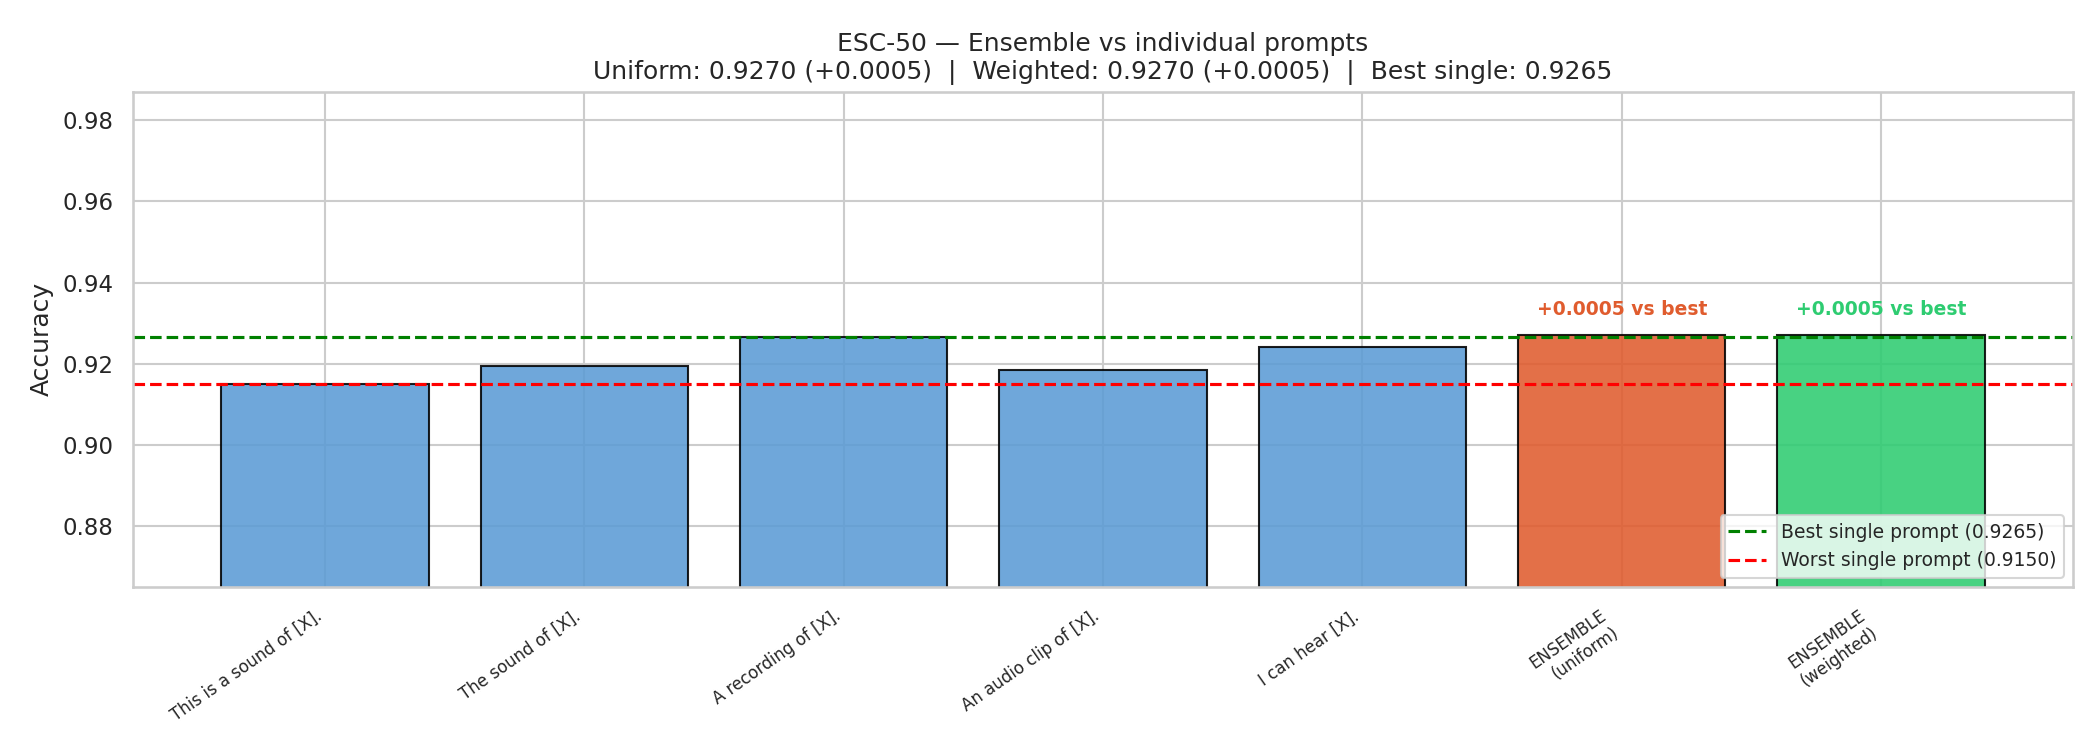
\includegraphics[width=\linewidth]{assets/figures/esc50/ensemble_comparison.png}
  \caption{\dataset{ESC-50}.}
\end{subfigure}
\hfill
\begin{subfigure}[t]{0.48\textwidth}
  \centering
  
\includegraphics[width=\linewidth]{assets/figures/urbansound8k/ensemble_comparison.png}
  \caption{\dataset{UrbanSound8K}.}
\end{subfigure}

\vspace{0.75em}

\begin{subfigure}[t]{0.48\textwidth}
  \centering
  
\includegraphics[width=\linewidth]{assets/figures/gtzan/ensemble_comparison.png}
  \caption{\dataset{GTZAN}.}
\end{subfigure}
\hfill
\begin{subfigure}[t]{0.48\textwidth}
  \centering
  
\includegraphics[width=\linewidth]{assets/figures/fsdd/ensemble_comparison.png}
  \caption{\dataset{FSDD}.}
\end{subfigure}
\caption{Ensemble comparison plots for all datasets.}
\end{figure}

\subsubsection*{Confusion Matrices}

\begin{figure}[H]
\centering
\begin{subfigure}[t]{0.48\textwidth}
  \centering
  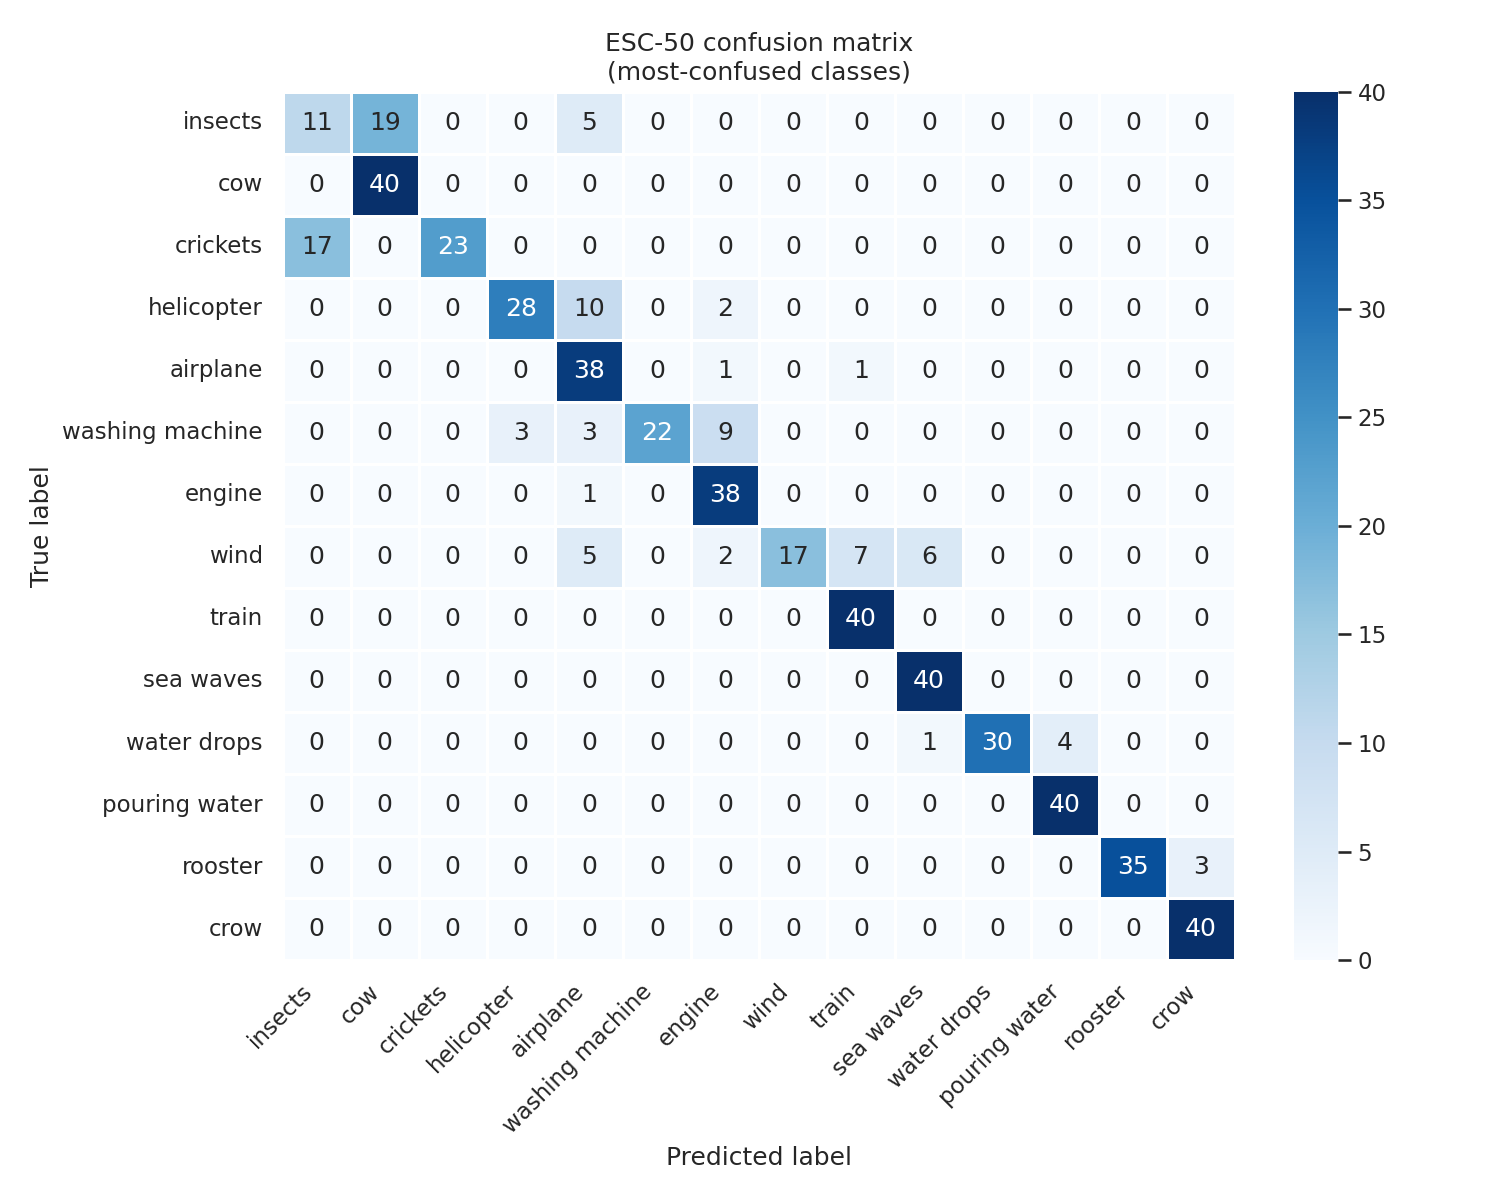
\includegraphics[width=\linewidth]{assets/figures/esc50/confusion_matrix.png}
  \caption{\dataset{ESC-50}.}
\end{subfigure}
\hfill
\begin{subfigure}[t]{0.48\textwidth}
  \centering
  
\includegraphics[width=\linewidth]{assets/figures/urbansound8k/confusion_matrix.png}
  \caption{\dataset{UrbanSound8K}.}
\end{subfigure}

\vspace{0.75em}

\begin{subfigure}[t]{0.48\textwidth}
  \centering
  
\includegraphics[width=\linewidth]{assets/figures/gtzan/confusion_matrix.png}
  \caption{\dataset{GTZAN}.}
\end{subfigure}
\hfill
\begin{subfigure}[t]{0.48\textwidth}
  \centering
  
\includegraphics[width=\linewidth]{assets/figures/fsdd/confusion_matrix.png}
  \caption{\dataset{FSDD}.}
\end{subfigure}
\caption{Confusion matrices for all four datasets.}
\end{figure}

The confusion matrices reinforce the metric-level story. \dataset{GTZAN}
errors cluster among related genres, while \dataset{FSDD} shows broad confusion
across digit classes and no strong zero-shot structure.

\subsubsection*{Prompt Sensitivity Plots}

\begin{figure}[H]
\centering
\begin{subfigure}[t]{0.48\textwidth}
  \centering
  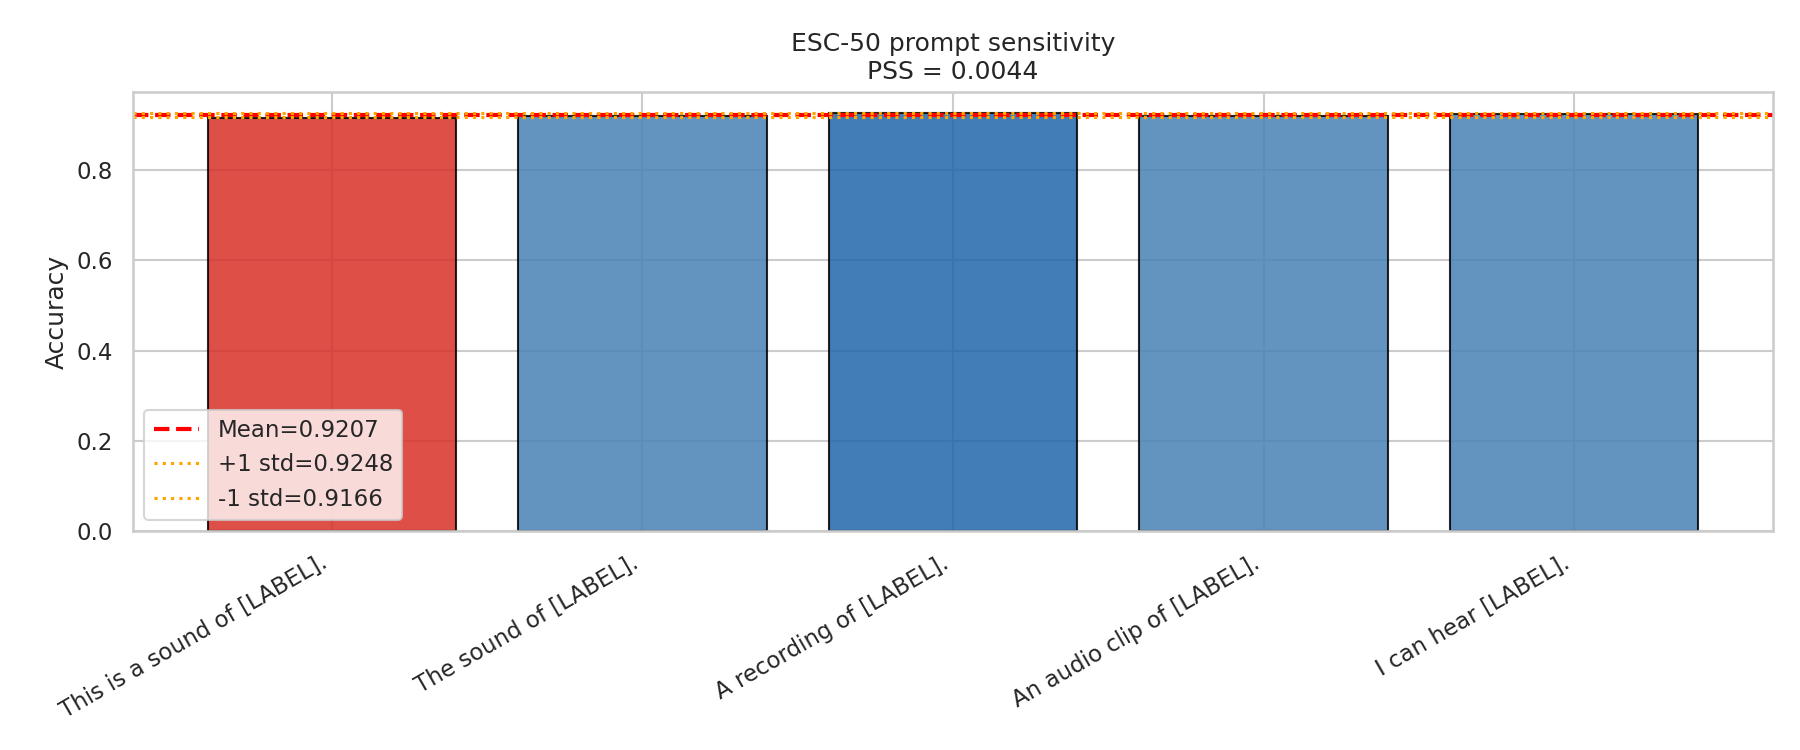
\includegraphics[width=\linewidth]{assets/figures/esc50/prompt_sensitivity.png}
  \caption{\dataset{ESC-50}.}
\end{subfigure}
\hfill
\begin{subfigure}[t]{0.48\textwidth}
  \centering
  
\includegraphics[width=\linewidth]{assets/figures/urbansound8k/prompt_sensitivity.png}
  \caption{\dataset{UrbanSound8K}.}
\end{subfigure}

\vspace{0.75em}

\begin{subfigure}[t]{0.48\textwidth}
  \centering
  
\includegraphics[width=\linewidth]{assets/figures/gtzan/prompt_sensitivity.png}
  \caption{\dataset{GTZAN}.}
\end{subfigure}
\hfill
\begin{subfigure}[t]{0.48\textwidth}
  \centering
  
\includegraphics[width=\linewidth]{assets/figures/fsdd/prompt_sensitivity.png}
  \caption{\dataset{FSDD}.}
\end{subfigure}
\caption{Prompt sensitivity across all datasets.}
\end{figure}

These plots show that prompt wording matters more on some datasets than others,
which helps explain why ensembling can fail: averaging can dilute the signal of
the best prompt.

\subsubsection*{Reliability Diagrams}

\begin{figure}[H]
\centering
\begin{subfigure}[t]{0.48\textwidth}
  \centering
  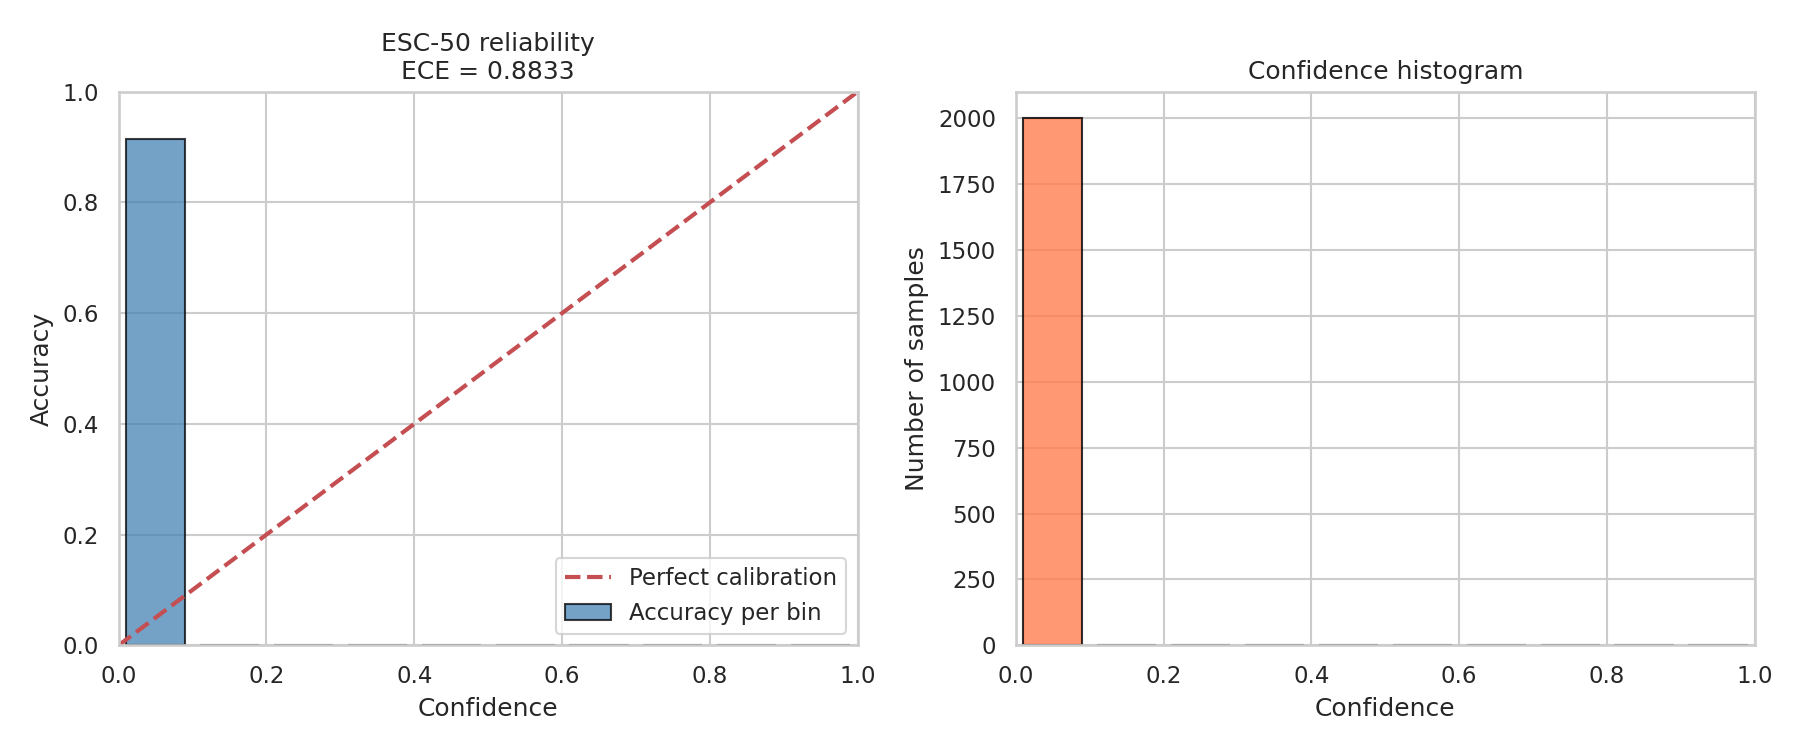
\includegraphics[width=\linewidth]{assets/figures/esc50/reliability.png}
  \caption{\dataset{ESC-50}.}
\end{subfigure}
\hfill
\begin{subfigure}[t]{0.48\textwidth}
  \centering
  
\includegraphics[width=\linewidth]{assets/figures/urbansound8k/reliability.png}
  \caption{\dataset{UrbanSound8K}.}
\end{subfigure}

\vspace{0.75em}

\begin{subfigure}[t]{0.48\textwidth}
  \centering
  
\includegraphics[width=\linewidth]{assets/figures/gtzan/reliability.png}
  \caption{\dataset{GTZAN}.}
\end{subfigure}
\hfill
\begin{subfigure}[t]{0.48\textwidth}
  \centering
  
\includegraphics[width=\linewidth]{assets/figures/fsdd/reliability.png}
  \caption{\dataset{FSDD}.}
\end{subfigure}
\caption{Reliability diagrams for all datasets.}
\end{figure}

\subsubsection*{Per-Class Accuracy}

\begin{figure}[H]
\centering
\begin{subfigure}[t]{0.48\textwidth}
  \centering
  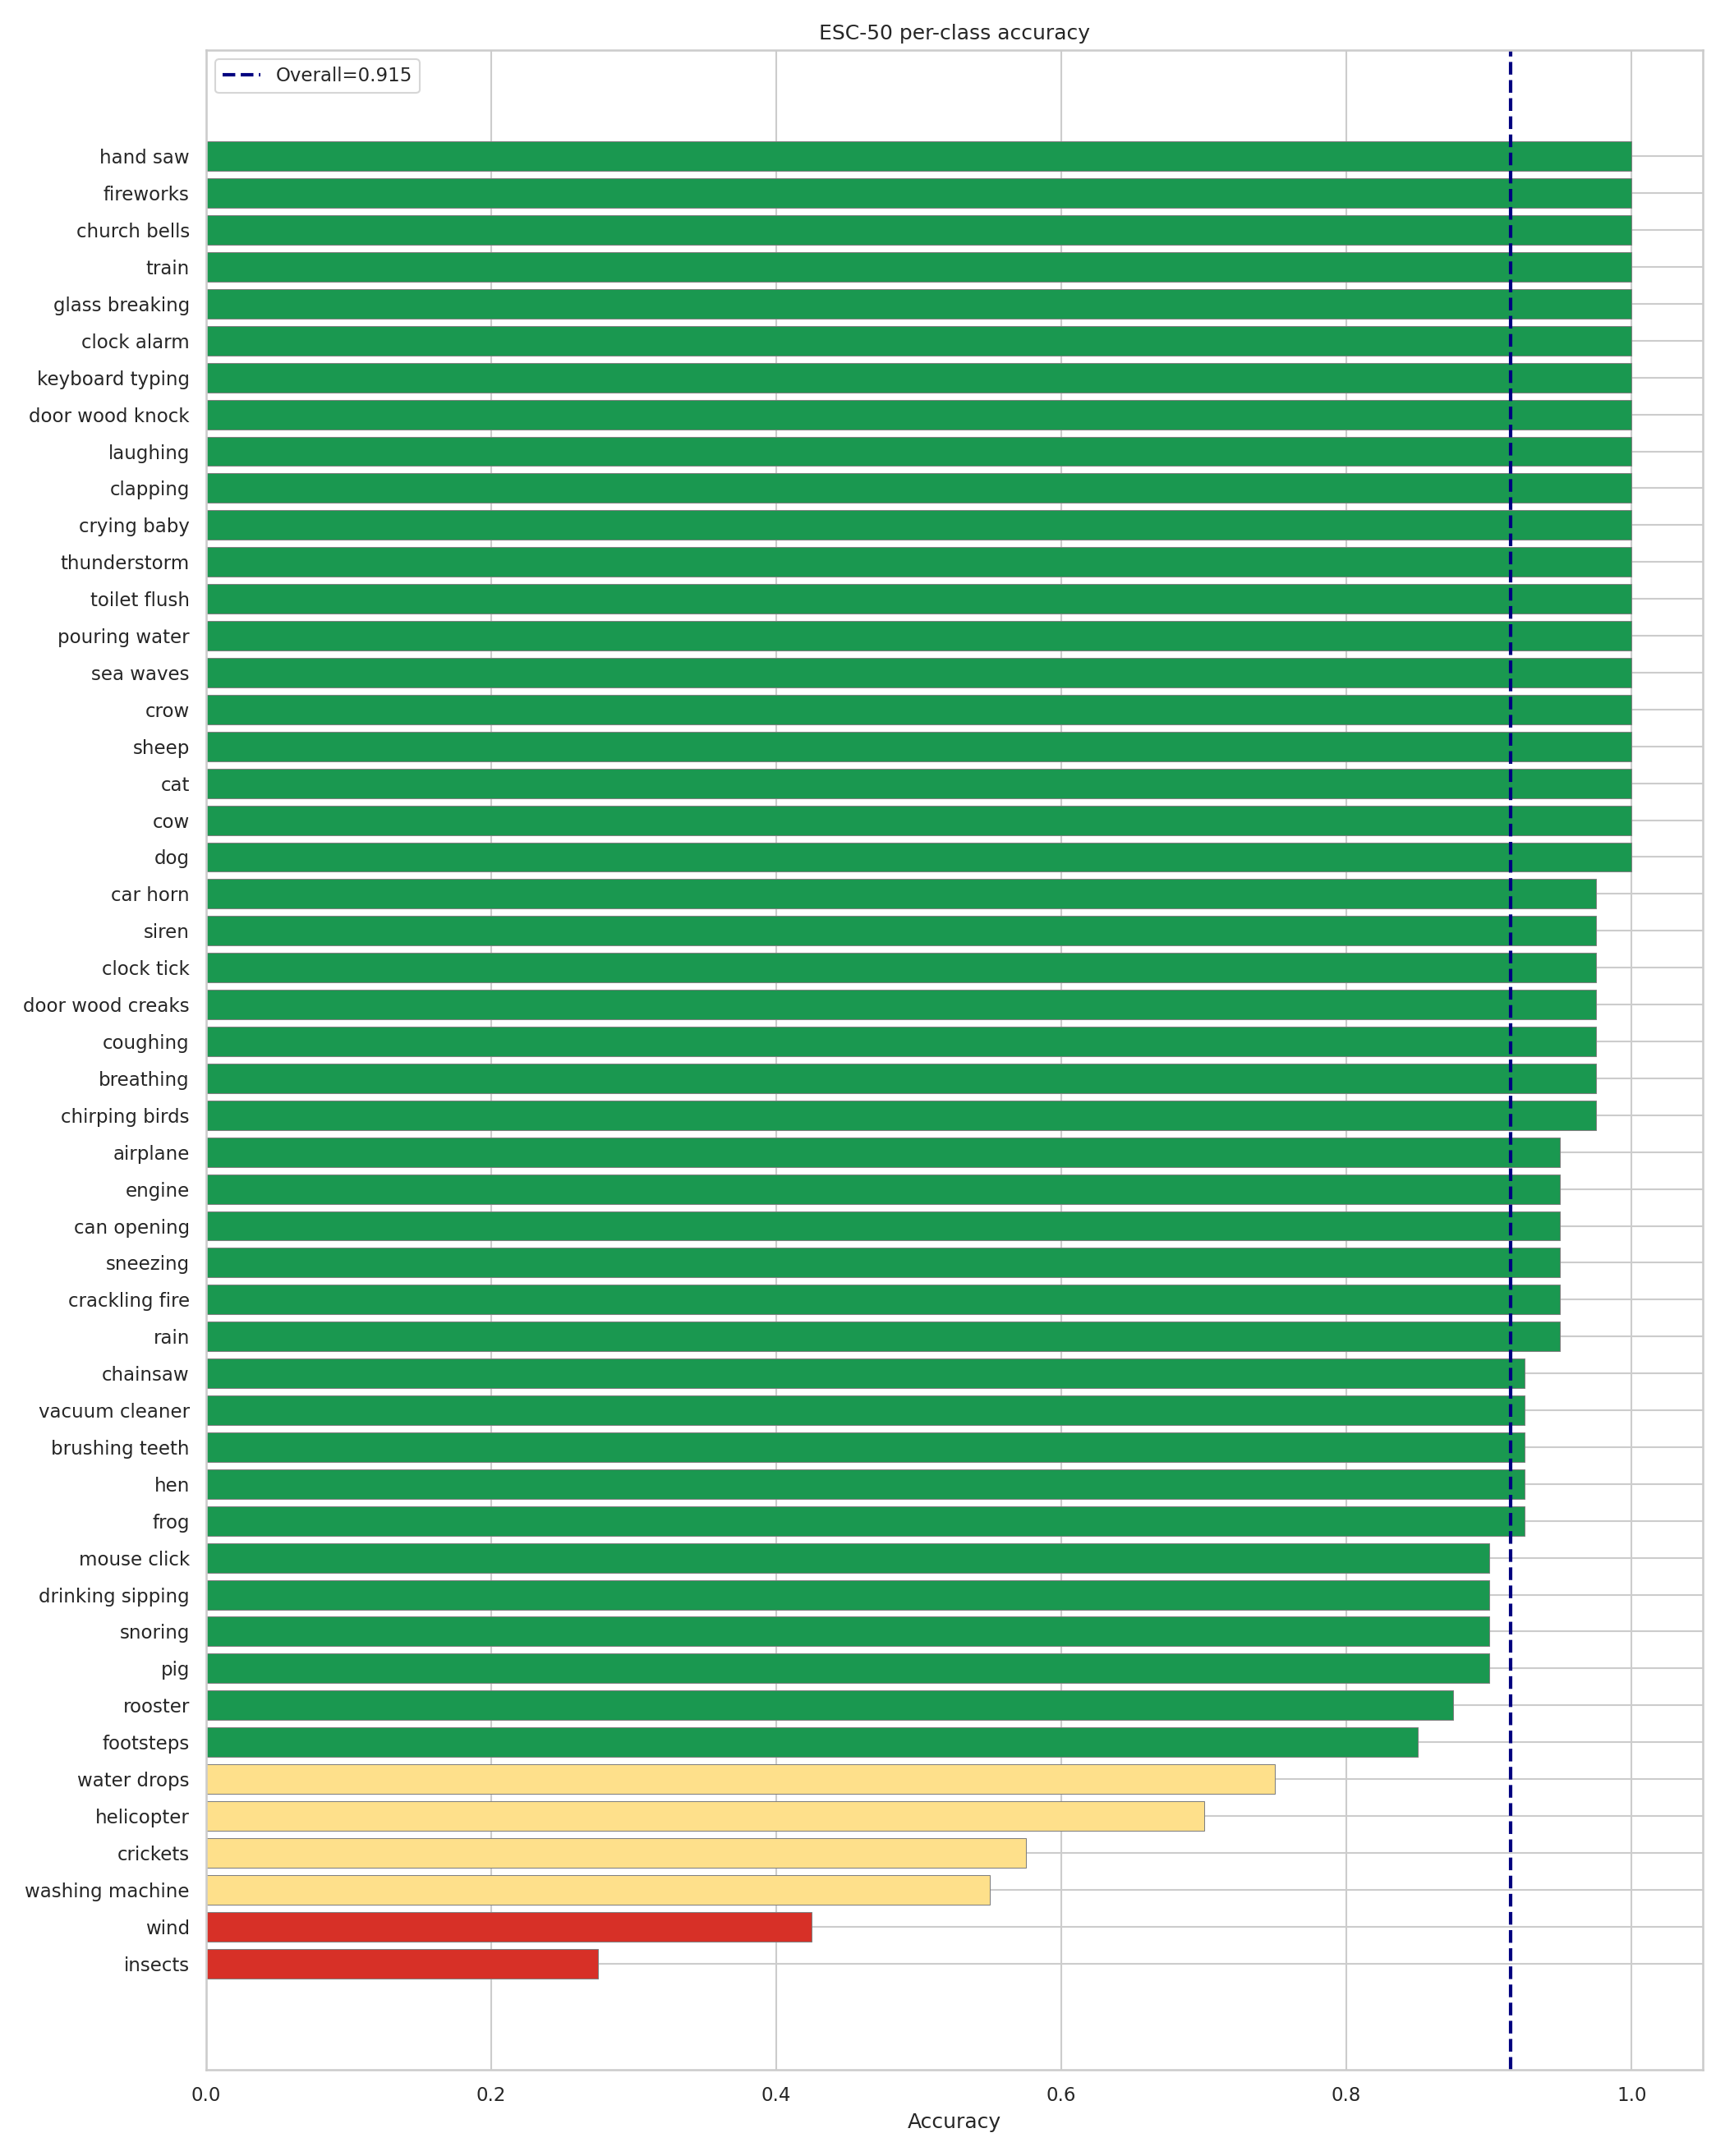
\includegraphics[width=\linewidth]{assets/figures/esc50/per_class_accuracy.png}
  \caption{\dataset{ESC-50}.}
\end{subfigure}
\hfill
\begin{subfigure}[t]{0.48\textwidth}
  \centering
  
\includegraphics[width=\linewidth]{assets/figures/urbansound8k/per_class_accuracy.png}
  \caption{\dataset{UrbanSound8K}.}
\end{subfigure}

\vspace{0.75em}

\begin{subfigure}[t]{0.48\textwidth}
  \centering
  
\includegraphics[width=\linewidth]{assets/figures/gtzan/per_class_accuracy.png}
  \caption{\dataset{GTZAN}.}
\end{subfigure}
\hfill
\begin{subfigure}[t]{0.48\textwidth}
  \centering
  
\includegraphics[width=\linewidth]{assets/figures/fsdd/per_class_accuracy.png}
  \caption{\dataset{FSDD}.}
\end{subfigure}
\caption{Per-class accuracy plots for all datasets.}
\end{figure}

\section{Discussion}

The project produces a balanced scientific picture of CLAP:
\begin{itemize}[leftmargin=1.25em]
  \item it is genuinely strong on environmental sound recognition;
  \item it remains useful on urban sound recognition;
  \item it is workable but limited on music genre classification;
  \item it is weak on fine-grained spoken-digit recognition.
\end{itemize}

The most important insight is that CLAP's transfer ability is
\textbf{domain-sensitive}, not uniformly strong.

Three points are especially important in the final write-up:
\begin{itemize}[leftmargin=1.25em]
  \item the benchmark reproduction was successful, but it uses a stronger
  checkpoint than the one emphasized in the original comparison;
  \item richer metrics provide a more honest description than top-1 accuracy
  alone;
  \item prompt ensembling should be reported as a validated negative result
  rather than as a successful improvement.
\end{itemize}

\subsection{What Should Be Claimed in the Final Submission}

The strongest claims supported by the final run are:
\begin{itemize}[leftmargin=1.25em]
  \item The benchmark suite \dataset{ESC-50}, \dataset{UrbanSound8K}, and
  \dataset{GTZAN} was reproduced in a verified WSL pipeline.
  \item The final benchmark uses the stronger
  \dataset{630k-audioset-best.pt} checkpoint, so it should be described as an
  improved-checkpoint reproduction rather than a strict same-checkpoint
  replication.
  \item \dataset{FSDD} was added as a new diagnostic dataset.
  \item Multiple richer metrics were added beyond plain accuracy.
  \item Prompt ensembling was implemented and evaluated.
  \item Prompt ensembling does not reliably improve CLAP.
  \item Entropy-weighted prompt ensembling collapses to effectively uniform
  behavior.
  \item CLAP transfers poorly to zero-shot spoken-digit recognition on
  \dataset{FSDD}.
\end{itemize}

\subsection{Limitations}

\begin{itemize}[leftmargin=1.25em]
  \item The final benchmark comparison is not a strict same-checkpoint
  replication of the original paper.
  \item The environment had to be stabilized to a working CUDA-compatible WSL
  stack, so the exact package mix should be treated as part of the reported
  method.
  \item \dataset{GTZAN} required explicit raw-data conversion from
  \dataset{.au} to \dataset{.wav} and removal of the known corrupted sample.
  \item The extension conclusions are strong empirically, but they are still
  bounded by the prompt families and checkpoint used in this study.
\end{itemize}

\section{Conclusion}

This project delivered:
\begin{itemize}[leftmargin=1.25em]
  \item a verified CLAP benchmark run over four datasets,
  \item a reproducible WSL execution setup,
  \item richer evaluation metrics,
  \item a new diagnostic dataset,
  \item a clear extension study on prompt ensembling.
\end{itemize}

The main final message is balanced rather than purely celebratory: CLAP is
genuinely strong for some zero-shot audio tasks, but its gains are uneven
across domains, and prompt ensembling is not a dependable shortcut to better
performance. That combination of successful reproduction, practical
engineering, and validated negative-result analysis makes this project stronger
than a plain rerun of the original benchmark.

\end{document}
